\documentclass{article}
\usepackage[utf8]{inputenc}
\usepackage[margin=1.2in]{geometry}

%Package enabling roman numerals in lists
\usepackage{enumitem}

%Package enabling dashed lines
\usepackage{arydshln}

%Package to show images
\usepackage{graphicx}
\graphicspath{ {./images/} }

%Package to display requirements as in SRS
\usepackage{tabularx}

\title{Architecture Notebook}

\author{Jonas Malm}
\date{Fall 2020\\---\\Version 0.8.2}

\begin{document}

\maketitle
\clearpage

\newgeometry{margin=0.7in}
\begin{table}
\section*{Version history}
\centering
\begin{tabular}{|l|l|l|l|}
\hline
Version & Date & Author & Description \\ \hline
0.1.0 & 2020-10-15 & Jonas Malm & Creation of document\\ 
0.2.0 & 2020-10-16 & Jonas Malm & Added architectural goals, finished ASRs\\
0.2.1 & 2020-11-02 & Jonas Malm & Added architectural constrains\\ 
0.3.0 & 2020-11-02 & Jonas Malm & Added architectural decisions\\
0.3.1 & 2020-11-04 & Jonas Malm & Refined decisions and ASRs\\
0.4.0 & 2020-11-04 & Jonas Malm & Added key abstractions and started layers\\
0.4.1 & 2020-11-05 & Jonas Malm & Wrote detailed layers\\
0.4.2 & 2020-11-09 & Jonas Malm & Added a glossary\\
0.4.3 & 2020-11-09 & Jonas Malm & Mades revisions based on feedback from Gustaf Eriksson\\
0.4.4 & 2020-11-09 & Jonas Malm & Re-wrote ASR to facilitate traceability\\
0.5.0 & 2020-11-10 & Jonas Malm & Added user cases\\
0.5.1 & 2020-11-10 & Jonas Malm & Modified box and line to separate filtration module\\
0.5.2 & 2020-11-10 & Jonas Malm & Added overview sequence diagram\\
0.6.0 & 2020-11-11 & Jonas Malm & Started work on the authentication section\\
0.6.1 & 2020-11-12 & Jonas Malm & Added new section to arch. decisions: Using Auth0\\
0.6.2 & 2020-11-13 & Jonas Malm & Added subsection to AD: Role-based access control\\
0.6.3 & 2020-11-13 & Jonas Malm & Added RBAC Roles to authentication section\\
0.6.4 & 2020-11-13 & Jonas Malm & Added an authentication sequence diagram\\
0.6.5 & 2020-11-13 & Jonas Malm & Added Patient View sequence diagram\\
0.6.6 & 2020-11-16 & Jonas Malm & Added Placement of modules in Arch. dec. section\\
0.7.0 & 2020-11-16 & Jonas Malm & Wrote the scaleability in future section\\
0.7.1 & 2020-11-18 & Jonas Malm & Wrote the support in future section\\
0.7.2 & 2020-11-18 & Jonas Malm & Started maintainability in future section\\
0.7.3 & 2020-11-18 & Jonas Malm & More maintainabillity: more data and replacing EhrScape\\
0.7.4 & 2020-11-20 & Jonas Malm & Fixed inconsistencies in how HCU were named\\
0.8.0 & 2020-11-20 & Jonas Malm & Future dev: Added trend analysis and two figures\\
0.8.1 & 2020-11-22 & Jonas Malm & Future dev: Added advanced notification log and one figure\\
0.8.2 & 2020-11-22 & Jonas Malm & Future dev: Added tweaking rule engine\\


\hline
\end{tabular}
\end{table}
\restoregeometry

\textbf{TODO:}
\begin{enumerate}[label=(\roman*)]
\item Write dependencies
\item Add deployment view
\item Finish work on authentication
\item Update ASRs when requirements are re-numbered
\item Populate appendix
\item Run tests on the Rule Engine and Filtration Module in order to determine how performance is affected by number of patients
\end{enumerate}


\clearpage

\tableofcontents
\clearpage

\section{Introduction}
\subsection{Purpose}
This document describes the software architecture of the system. Furthermore it describes the software modules that will be built and incorporated into the system, and delivers an overview of their function as well as an description of how they will support the project's goals.

\subsection{Definitions, acronyms and abbreviations}
\begin{description}
\item [EHR] An \emph{Electronic Health Record} is a record containing patient health data in an electronic form.
\item [OpenEHR] is a collection of open industry specifications, models and software for e-health.
\item [AQL] The \emph{Archetype Query Language} is a declarative query language developed to search and retrieve data in archetype-based repositories, such as an OpenEHR-database.
\item [HCU] An abbreviation of Health Care Unit.
\item [OAuth] An open standard for authorization delegation. It allows a service owner to allow third-party server access without sharing credentials, instead using access tokens. 
\item [RBAC] Role-Based Access Control is a way to assign access levels based on what role a user has.
\end{description}

\subsection{Goal of the project}
The key goal of HeartByte's product is to provide health care providers an easy-to-use system to monitor and care for a large group of patient with limited resources. Thus the architecture of this software contains modules that enable health care providers to gain an overview over a large group of patient while identifying key patients through autonomous classification and manual filtration and sorting, as well as supporting components.

\subsection{Architectural goals}
The goal of the architecture is to reach the project goal while fulfilling a few software specific goals. The customer has expressed a wish that the software be designed and build in accordance to the aspects below.

\subsubsection{Achieving high modularity with pre-built components}
The customer, Region Östergötland, wants to be able to combine parts from different systems together. In order for it to be possible to combine parts of HeartByte's software with parts from other systems, the software needs to be designed in a way so it maintains a high degree of modularity and a high degree of cohesion within modules. Otherwise combining functionality from HeartByte's software with other systems would be very difficult. Using pre-built, standardized components further enables this, since they are easily replaced and modular by definition.

\subsubsection{Ensuring integration with existing systems is easy}
In order to facilitate a simple integration process into existing systems the architecture needs to take existing systems into consideration. This includes loading and storing patient data in the same format as existing systems, loading and storing care giver data in the same format as existing systems and using the same kind of authentication method.

\subsubsection{Creating software independent of OS and platform}
Furthermore, the customer wants a system that can be used from different operating systems as well as platforms. Some care givers might use tablets running iOS while others use Android and others still use a computer or even a smartphone. In conclusion it is important for the customer that the system can be accessed and used from a multitude of OSs and platforms, which will have implications on the architecture and the choice of stack. 



\subsection{Architectural constraints}
Due to the nature of the project, there are several constraints which have to be considered. Most importantly, the time frame and the skills of the development team.

\subsubsection{Time constraint}
According the the project plan, the project is to be finished in about three months. The first month, iteration 0 and 1, is spent setting up an organizational structure, communicating with the customer to elicit needs and creating requirements and then one week of education for the development team. Then there are two weeks of developing in iteration 2, two weeks in iteration 3 and one week in iteration 4. 
Thus there are only five weeks where the system is to be developed. If the project is to be completed on time, these five weeks will have to be used effectively. The architecture of the system will have to reflect this and thus focus on creating the modules that add the most value to the customer, while using pre-built components as much as possible.

\subsubsection{Skill constraint}
Since there is only one week for educating the development team, the choice of stack will have to reflect this and try to leverage existing knowledge over creating new. According to the skill set study by \emph{Configuration Manager Sam Anlér}, the team is proficient in these languages:

\begin{table}[h]
\centering
\begin{tabular}{|l|l|l|}
\hline
Language & Number of proficient users & Share of team \\ \hline
Java & 23 & 88\% \\
HTML & 20 & 77\% \\ 
JavaScript & 18 & 69\% \\ 
SQL & 18 & 69\% \\ 
Python & 15 & 58\% \\ 
\hline
\end{tabular}
\end{table}



\subsection{Assumptions and dependencies}
\subsubsection{Assumptions}
\begin{enumerate}[label=(\roman*)]
\item The system will not be used on mobile devices, thus platform and OS independence applies only to computers and tablets 
\item The customer uses a openEHR system to store EHRs, and the same templates as 
\item The rules used in the rule engine are set by the HCUs admin and not by HeartByte. HeartByte thus cannot take responsibility over if scientifically correct rules are applied, only that the patients are prioritized according to them.
\end{enumerate}
\subsubsection{Dependencies}


\section{Architecturally significant requirements}
Listed below are the Architecturally significant requirements (ARSs), the requirements most central to the architectural design. 

\subsection{Patient views}
\begin{tabularx}{\linewidth}{| l | X |}
 \hline
 \textbf{ID:} & FR007  \\ 
 \hline
 \textbf{Statement:} & The user shall be able to shift between a "patient view" where many patients are shown and a "overview view" where only one patient are shown. \\
 \hline
\end{tabularx}
\\ \\

Below, ASRs concerning these two views will be presented.

\subsubsection{Patient overview}
\begin{tabularx}{\linewidth}{| l | X |}
 \hline
 \textbf{ID:} & FR009  \\ 
 \hline
 \textbf{Statement:} & The admin shall be able to specify the variables that affects the health prioritization. The system shall provide the possibility to specify different variables for different health care units. 
 \\ 
 \hline
 
 \textbf{ID:} & FR004  \\ 
 \hline
 \textbf{Statement:} & The system shall display all patients in preferred order to a user who sort patients by [age, alert-level, measurements, health care unit, team, disease and patients’conditions]. \\ 
 \hline
 
 \textbf{ID:} & FR003  \\ 
 \hline
 \textbf{Statement:} & The system shall display all matching patients to a user who filter patients by [age, alert-level, measurements, health care unit, team, disease and patients’conditions]. \\ 
 \hline

 \textbf{ID:} & FR011  \\ 
 \hline
 \textbf{Statement:} & The admin shall be able to customize and save different views of the system. (e.g. a predefined view over diabetes patients who are over 30 years)
  \\ 
 \hline
\end{tabularx}
\\ \\

The requirements state that the software shall have an overview of patients where a health care provider can:
\begin{enumerate}[label=(\roman*)]
\item prioritize patients assisted by a module implementing care unit-specific triage rules,
\item sort patients,
\item filter patients based on multiple criteria,
\item save and load these filter views for later use.
\end{enumerate}
Thus a rule engine will be implemented that loads rule sets created by an admin as well as a database storing custom filter views and custom rules.


\subsubsection{Patient view}

\begin{tabularx}{\linewidth}{| l | X |}
 \hline
 \textbf{ID:} & FR026  \\ 
 \hline
 \textbf{Statement:} & In the view of a patient user shall be able to see personal information (gender, age occupation, social security number) 
 \\ 

 \hline
 \textbf{ID:} & FR043  \\ 
 \hline
 \textbf{Statement:} & In the overview of a patient the user shall at the top of the view be presented with the patient’s current medication(s).
 \\ 
 \hline

 \hline
 \textbf{ID:} & FR044  \\ 
 \hline
 \textbf{Statement:} & In the overview of a patient the user shall at the bottom of the view be presented with responsible healthcare provider(s) and associated hospital or clinic.
 \\ 
 \hline
\end{tabularx}
\\ \\

The requirements state that detailed information about a patient from his or her EHR is to be displayed in a dedicated view for the specific patient. This information includes current medications, next of kin, health data as well as a calendar visualizing upcoming events for the patient.

\subsubsection{Format}
\begin{tabularx}{\linewidth}{| l | X |}
 \hline
 \textbf{ID:} & NFR013  \\ 
 \hline
 \textbf{Statement:} & The system shall enable use of openEHR platforms as storage backend for EHR content (e.g. measurements, content from forms filled out by the patient and care plan).
 \\ 
 \hline
\end{tabularx}
\\ \\

The requirements further stipulate that all patient \emph{Electronic Health Records}, EHRs, have to be stored and loaded from databases in accordance with the \emph{openEHR open standard specification}. This is furthermore of great importance to the customer, since they cannot integrate the software with its existing software and servers without the key requirement being fulfilled.

\subsubsection{Patient data and access}

\begin{tabularx}{\linewidth}{| l | X |}
 \hline
 \textbf{ID:} & FR038  \\ 
 \hline
 \textbf{Statement:} & The user shall only get access to the data if the user chooses to access it
  \\ 
 \hline

 \textbf{ID:} & FR006  \\ 
 \hline
 \textbf{Statement:} & The system shall notify the user if they tries to access patient data that they don't have authority to view.\\ 
 \hline

 \textbf{ID:} & FR008  \\ 
 \hline
 \textbf{Statement:} & The system shall log which users who viewing which patients. These activities shall be saved in a log file.
\\ 
 \hline

 \textbf{ID:} & NFR002  \\ 
 \hline
 \textbf{Statement:} & OAuth shall be used for login and authentication.
 \\ 
 \hline
\end{tabularx}
\\ \\

Health records are highly regulated and one important aspect is who is allowed to see what patient data. Thus the requirements state that the software shall save logs when a user accesses EHRs. The requirements also state that the users have to authenticate themselves using OAuth. 
Thus the following modules need to be implemented:

\begin{enumerate}[label=(\roman*)]
\item A database storing access logs
\item A database storing which Health Care Unit (HCU) a user belongs to, so it can be determined if a user has authority to access
\item An authentication system using OAuth
\end{enumerate}



\section{Architectural decisions}
Below are the most important architectural decisions listed, stemming from the architectural goals, the architectural constraints and the ASRs.

\subsection{Using a back end}
In order to accommodate the two database mentioned in the \emph{Access ASR}, a back end containing the access log and personnel databases needs to be implemented. This is because in order to ensure that EHRs are not served to unauthorized clients, the calls to the actual EHR Database will have to go through a server that logs access. Doing this client side would not be as secure since a modified client could simply bypass the logging or not validate access levels through the personnel database.

\subsection{Choice of front end stack}
The front end will be developed using the JavaScript framework ReactJS. This is due to a few reasons:

\begin{enumerate}[label=(\roman*)]
\item By building a web app and using React, \emph{platform and OS independence} is enabled.
\item Due to the skill constraint, we want to leverage existing knowledge. The team is proficient in JavaScript and \emph{React is a JavaScript framework}.
\item Due to the time constraint, we need a language that is \emph{quick to learn and simple to use}. This holds true for React, which due to its wide spread use has many tutorials and good documentation.
\item One of the architectural goals is to achieve \emph{high modularity through reusable components}. React facilities this through allowing developers to split the UI into independent components and there are many free open-source components because of the popularity of the framework enabling quick development.
\end{enumerate}

\subsection{Choice of back end stack}
Due to the time and skill constraints, this back end and the databases would ideally leverage existing knowledge in the team. The back end will be developed in Python, using the web framework Flask for the server and the framework SQL Alchemy for the databases. The rationale behind these decisions is explained below.

\subsubsection{Python}
Python is a language that is easy to work with and easy to read; is easy to read, very popular as a back end language which ensures good help and has many web application frameworks. Since a majority of the team already are familiar with Python and the reasons listed above it is a good choice for back end. 
\subsubsection{Flask}
The Flask web framework is easy to use, flexible and allows for unit testing through integrated support and a quick debugger. Furthermore some members of the team are already familiar with Flask, so it is a good choice as web framework.
\subsubsection{SQL Alchemy}
Since members are experienced with SQL and the back end will be developed in Python, a logical step is using the SQL Alchemy framework in order to make the database development faster. There are also members of the team that are familiar with this framework.

\subsection{Using EhrScape}
As specified in the ASRs, the patient EHRs must be stored using the openEHR standard. Due to the time constraint and the skill constraint, the project does not have time to either train developers or to develop a server storing EHRs in accordance to the openEHR standard. In order to accommodate this requirement the project will instead use EhrScape, a health data platform. The platform contains tools for easy handling of clinical models, health data queries and vendor independent data storage. This is accessed through an API and data is stored on EhrScape's EHR server.

\subsection{Using Auth0}
As stated in the ASRs, the system has to implement OAuth for authentication. Due to the time and skill constraints as well as the scope of the project, developing a authentication system utilizing OAuth would not be a good decision. In order to facilitate integration with the customers current Identity Management solution, HeartByte will implement its authentication solution through the Auth0 service. Auth0 uses OAuth 2.0, which is supported by the customer's Identity Management solution and which will make the future integration easy. Through the Auth0 API, authentication can be handled from the HeartByte system and permission scopes can be quickly set up and managed from the Auth0 webpage.

\subsubsection{Role-Based Access Control}
The authentication system will implement RBAC. In RBAC you analyze the needs of users and group them into roles. Since patient access is based on what HCU you work at and some functionality is limited to admins, it is simple to split users into groups and to see what access roles these groups require.

\subsection{Placement of modules}\label{placement-modules}
Due to the security concerns presented above and due to some data being shared between all users, the databases and EHR Retriever will be placed in the back end. However, there are two more modules that have to be placed in either the front end or the back end: the Rule Engine prioritizing patients and the Filtration Module filtrating patients.

\subsubsection{Rule Engine}
The Rule Engine will be placed in the front end. This is due to that using a pure two-tier, thin-client would place a large workload on the back end if a large numbers of users request data at the same time. To avoid this the Rule Engine can be placed in the front end. 

\subsubsection{Filtration Module}
Some rudimentary filtration functionality will have to be implemented in the back end, when retrieving EHR data. Otherwise every user would receive the EHR data of all patients - even patients they are not treating. However, in order to minimize total loading time the main functionality will be placed in the front end. If all relevant patients are retrieved to the client and then applying the filtration, filtration will be faster. Otherwise many calls would have to be made to the back end. This would make the loading time longer since a call will have to be made to the back end and then the back end has to call the EhrScape Server.


\section{Key abstractions}
The key abstractions of the system is the front end, the back end and the EHR Database. The front end is what the user interacts with and the services supporting this. The back end contains the two databases and functionality to get data from these databases. The EHR Database is the external database storing the patient's EHR.

\begin{figure}[h]
    \centering
    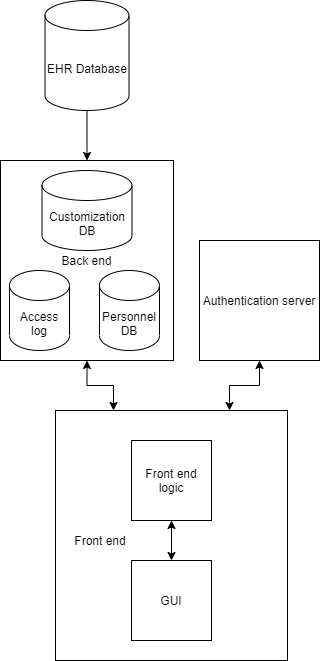
\includegraphics[scale = 0.5]{key-abstraction}
    \caption{The system and its key abstractions}
    \label{fig:key-abstractions}
\end{figure}


\subsection{Front end}
The main functionality of the front end is to create a way for the user to interact with and visualize patient data. The user will do this through the GUI, and the GUI will then communicate with the front end logic to enable the user to filter, sort and group patients. 

\subsection{Back end}
The back end serves the purpose set out in the in the ASRs and the architectural decisions. The back end will handle calls to the EHR Database and ensure that if a user accesses patients outside his or her patient group this is logged. The back end will also handle calls to the personnel database as well as storing the customization of the interface, patient views and rules for the rule engine.

\subsection{EHR Database}
The EHR Database is the database that store the patient EHRs. It will also store any custom AQL queries that are created to access the patient EHRs and templates used to store EHR data.


\section{Architectural views}
\subsection{User cases}
\begin{figure}[h]
    \centering
    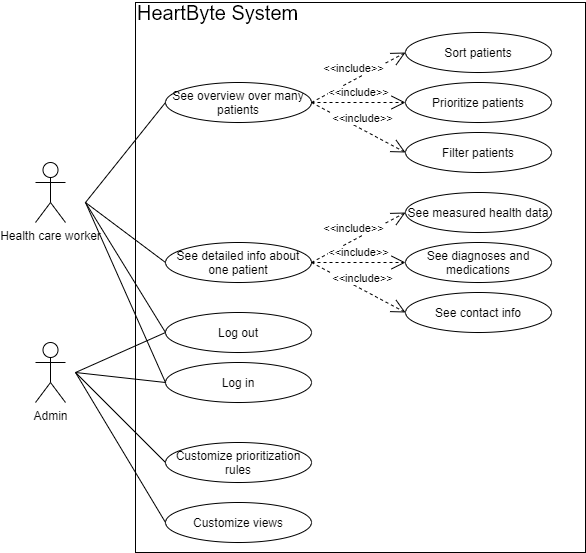
\includegraphics[scale = 0.5]{user-cases}
    \caption{Significant system user cases}
    \label{fig:user-cases}
\end{figure}

In Figure \ref{fig:user-cases} above, some of the more central user cases are illustrated. They are not exhaustive, but are presented to provide some context for the architectural design.

\subsection{System layers}
This section will describe components of the system in a detailed way through four layers: the GUI, the Front End Logic, the HeartByte Server and the EhrScape Server. The direction of the arrows indicate the direction of data flow.

\begin{figure}[h]
    \centering
    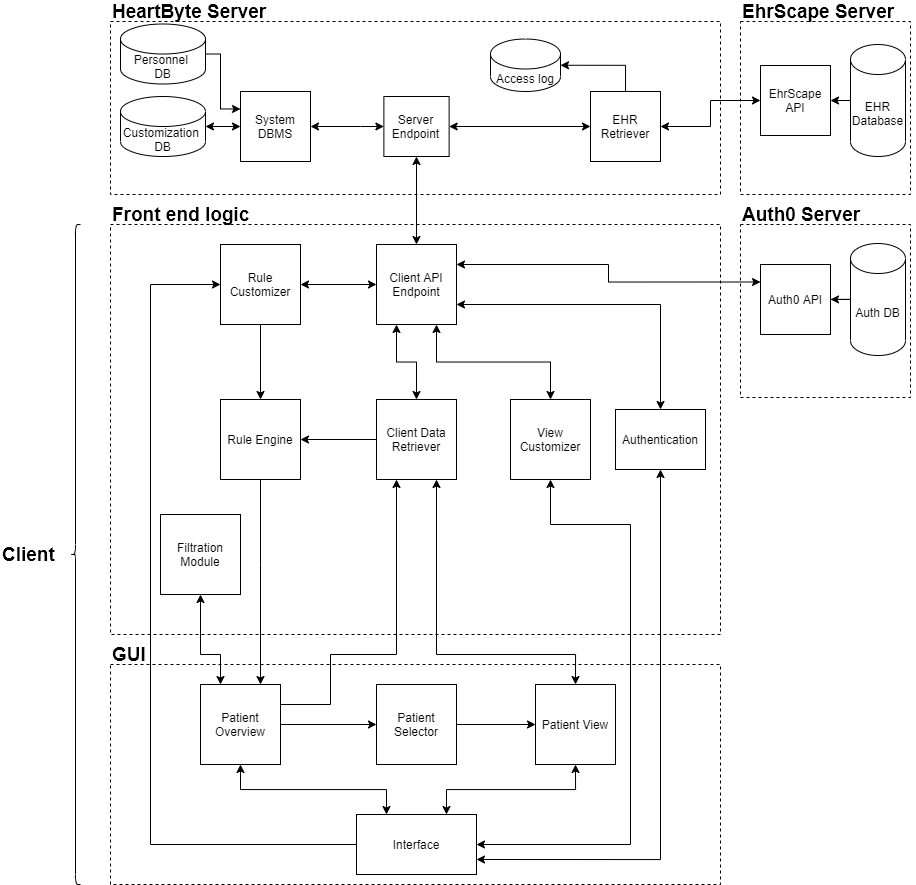
\includegraphics[scale = 0.45]{box-and-line}
    \caption{A box and line diagram illustrating layers of the system and its submodules}
    \label{fig:execution-view}
\end{figure}

As seen in Figure \ref{fig:execution-view}, the front end and back end interface will utilize the facade design pattern, so coupling and modularity is ensured. Below, the modules in the figure will be described by layer.

\subsubsection{GUI Layer}
The GUI consists of four main modules. The Interface is what the user will interact with and what will display the web app. From the Interface the user can access the Patient Overview, displaying many patients, and through the Patient Selector select a specific patient to be displayed in the Patient View. 

The Interface also allows a user to log in and for superusers, to customize the rules applied in the Rule Engine through the Rule Customizer and views of the patients through the View Customizer.

\subsubsection{Front End Logic Layer}
The Front End Logic contains the "middleware" interacting with the HeartByte Server and the GUI to deliver data to the GUI. The most central module is the Client Data Retriever. This module will handle calls from Patient Overview to get general data about a group of patients and calls from Patient View to get detailed data about a specific patient. 

When Patient Overview makes a call to this module, the servers response is passed to the Rule Engine for classification of how critical the patients health status is. The classified data is then passed back to the Patient Overview. The Patient Overview can then make calls to the Filtration Module to change the filters applied to the data already retrieved. When the Patient View makes calls to the Client Data Retriever, the results returned from the server are passed directly to the Patient View.

This layer also contains the modules used for authentication as well as the customization a superuser can do. To customize classification rules, the Interface calls the Rule Customizer which in turn loads or stores rules in the Customization Database. The View Customizer works in the same fashion. The Authentication module will make a call to the Personnel Database to determine what role the user has, and thus what information should be displayed.

\subsubsection{HeartByte Server Layer}
The HeartByte Server contains the databases specific to the system and the functionality to retrieve EHRs. The System Database Management allows for storing and loading data in the Personnel Database and the Customization Database. These databases contain data about custom rules and views for specific HCUs and personnel data, respectively.

The EHR Retriever is the module responsible for loading data from EHRs. This module will recieve a call about what data to retrieve, make a call to the EhrScape Server to retrieve the requested data and return the data through the Server Endpoint. The EHR Retriever will also make a call to the Personnel Database in order to check if the user requesting the EHR data works at one of the HCUs responsible for the patient. If this is not the case, this will be added to the log entry in the Access Log database.

\subsubsection{EhrScape Server Layer}
This layer is a database stored on an external server, which is accessed using the EhrScape API. The API is queried using stored custom Archetype Query Language (AQL) queries as well as using its REST API. Since this is the openEHR database query language it is easy to substitute this layer with another openEHR server in the future.

\clearpage
\subsection{Authentication} \label{Authentication}
In this part the authentication functionality is discussed in further detail.

\subsubsection{Patients and HCUs}
\begin{figure}[h]
    \centering
    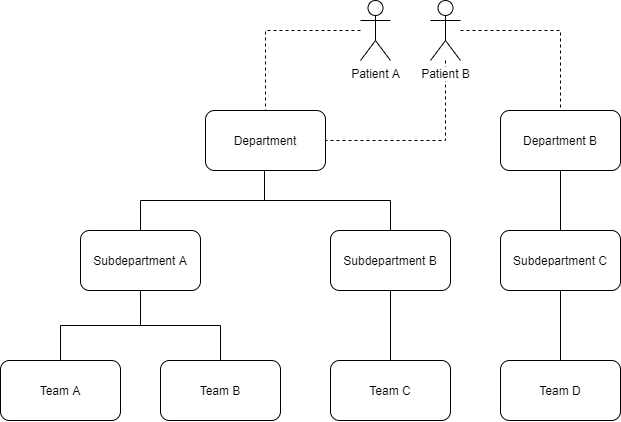
\includegraphics[scale = 0.45]{departments}
    \caption{A sequence diagram illustrating how the Patient Overview calls are handled by the system}
    \label{fig:departments}
\end{figure}

The users using the system belong to one or more groups. The structure of these groups are illustrated in the simple tree in Figure \ref{fig:departments}. An operation is a health care institution and could be e.g. a hospital or a health center, such as the Linköping University Hospital. These operations are divided into departments, such as Cardiology,  Infectious Diseases or Pediatrics. These departments are in turn comprised of teams.  
As illustrated, a patient is handled by one or many departments. Thus, a health care professional working at any department in Operation B is authorized to view the EHR of Patient B, but not the EHR of Patient A.
However, it is in the interest of the health care professionals working at Operation B to be able to access the EHR of Patient A, in case of an emergency. The system will facilitate this, but such accesses will be logged in the access log.

\subsubsection{RBAC Roles}
By analyzing the needs of users using the information above, they can be grouped and assigned access roles to be implemented in the RBAC system in Auth0.

\begin{description}
\item [Operation] The Operation role consists of several roles, one for each operation. A user that e.g. has the \emph{Operation A} role has access to the EHRs of all patients serviced by Operation A.
\item [Admin] The Admin role allows a user to make some customization changes for the other members in the same Operation as the user. This includes changing the rules used in the Rule Engine and adding custom filtered views, through accessing the modules Rule Customizer and View Customizer illustrated in Figure \ref{fig:execution-view}.
\end{description}


\subsection{Sequence diagrams}
In this section a few relevant sequence diagrams will be displayed, to further clarify how the modules will interact in typical user cases.

\subsubsection{Calls from the Overview module}
\begin{figure}[h]
    \centering
    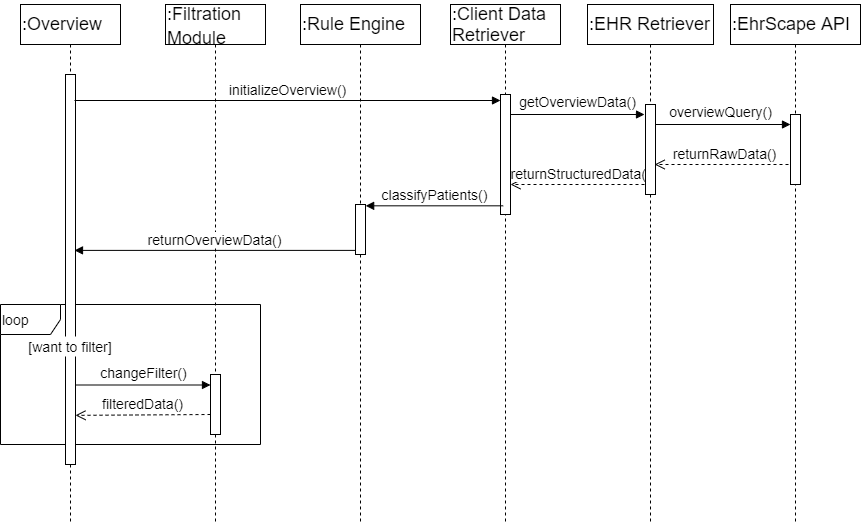
\includegraphics[scale = 0.45]{overview-sequence}
    \caption{A sequence diagram illustrating how the Patient Overview calls are handled by the system}
    \label{fig:overview-sequence}
\end{figure}

Worth noting from Figure \ref{fig:overview-sequence}, is that all relevant data is retrieved to the Overview. Once the data has been retrieved, filters can be applied without retrieving the data again. Since no sensitive data will be displayed to the user through the Overview, there is no need to log this in the access log.

\subsubsection{Calls from the Patient View module}
\begin{figure}[h]
    \centering
    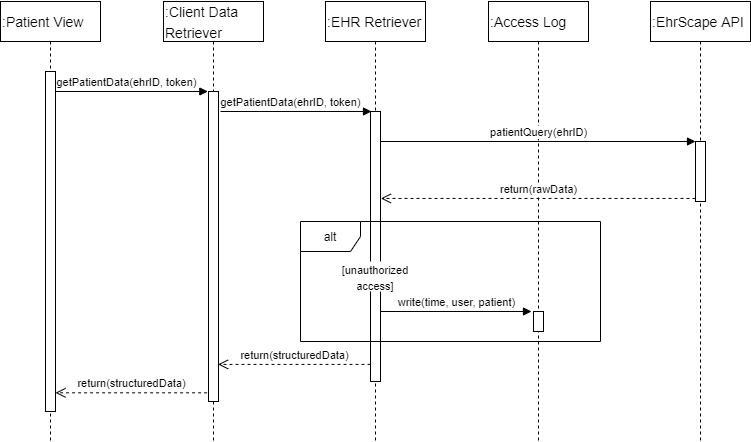
\includegraphics[scale = 0.45]{patient-sequence}
    \caption{A sequence diagram illustrating how the Patient View calls are handled by the system}
    \label{fig:patient-sequence}
\end{figure}

In Figure \ref{fig:patient-sequence}, EHR data about a specific patient is retrieved. The access token, with the user's access authentication from the role inside, is passed to the EHR Retriever. After retrieving the data about the requested patient, this module will compare the operation the patient belongs to with the role of the user from the access token. If these do not match, the access in unauthorized and this will be logged before structuring the returned data and passing it to the Patient View. Note that the data is returned even though the access is unauthorized, as specified in Section \ref{Authentication}. However, no data will be returned if the access token is invalid or missing.

\subsubsection{Authentication}
\begin{figure}[h]
    \centering
    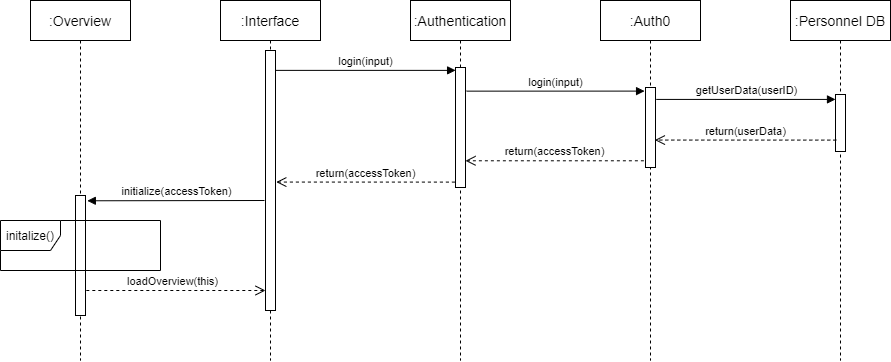
\includegraphics[scale = 0.45]{auth-sequence}
    \caption{A sequence diagram illustrating how authentication is handled}
    \label{fig:auth-sequence}
\end{figure}

As seen in Figure \ref{fig:auth-sequence}, Auth0 makes a request to the Personnel DB in the HeartByte server to get information about the user that logged in. Then this information is evaluated to assign one or several roles to the user. Then these roles are stored in the access token that is returned, that is required to access end points e.g. to load the Patient Overview.

\clearpage
\section{The system in the future}
\textbf{TODO:} 
This is only a stub, to be completed in the future

\subsection{Scaleability}
In this section the factors relevant to scaling the system up, in terms of number of patients and users, will be discussed.

\subsubsection{Prioritizing of large data sets}
The Rule Engine is placed in the Front end logic layer, as seen in Figure \ref{fig:execution-view}, due to the reasons outlined in section \ref{placement-modules}. The Rule Engine only prioritizes patients based on the most recent measurements, so the classification is not computationally heavy. Due to this, a large number of patients should not affect the performance of the system in a major way. This is not the case if the Rule Engine would implement more computationally heavy classification rules, as mentioned in section \ref{trend-analysis}.

However, with a very large data set and many patients displayed in the Patient Overview another potential problem would be created. If there are e.g. 100 patients displayed unfiltered, there might be many patients classified as high priority. Then it would not be easy to see which ones are the most relevant. This can be addressed by the user, in the existing system, by filtrating on some factors to reduce the number of displayed patients, but a potentially better solution is discussed in section \ref{future-prioritization}.

\subsubsection{Filtration of large data set}
Since the filtration functionality is placed in the front end, performance could be expected to suffer when working with very large data sets. The rationale laid out in section \ref{placement-modules} is based on assumptions of a moderately sized data set and frequent filtration. However, if the data set would be very large and the filtration isn't happening frequently then the rationale might not be valid. The time lost due to calls to the back end and EhrScape could be offset by time lost due to hardware limitations on the client side. It is considered unlikely that this will be the case however, since simple tests on larger sets of patients have not shown a drop in performance.

If however performance were to be affected due to a larger number of patients, the recommended solution would be to limit the number of patients that are returned to the overview. In the current implementation, all patients that the user has authority to access are returned. This could be changed so that only patients tended  to by the user's department or team are returned. To implement this, additional data fields in the demographic database in EhrScape could be added.

\subsubsection{Increasing the number of users}
Increasing the number of users should not affect the performance of the system, since the system is designed utilizing a two-tier fat-client where no computationally heavy functionality is implemented in the back end. 

\subsection{Support}
HeartByte will work alongside the customer to implement and integrate the system. Once the implementation is secured the operation of the system will be transferred to the customer. During the transfer process, members of the HeartByte development team will be deeply involved to ensure that the customer fully understands how the system is constructed. This, alongside the documentation will enable the operation of the system to be transferred to the customer. HeartByte will also provide some support during the first year after delivery of the product. This support includes answering questions and fixing any bugs shipped in the product.

\subsection{Maintaining}
This section will handle the topic of the maintaining of the system and extending with new functionality as needed. Because the system has been built with maintainability in mind though modularity, in most cases this is relatively simple. This is not true for all functionality though, as discussed below.

\subsubsection{Adding more health data}
As of now, the system is only built to handle a few selected health data points. These include weight, blood pressure and
physical activity. If more are to be added this would mean extending the functionality in the areas below.

\begin{description}
\item [openEHR Templates] If one does not already exist for the measurement, a new template will have to be constructed and added to EhrScape. Since the customer are experienced using the tools required to do this, this would not pose a significant challange.

\item [EHR Retriever] In the EHR Retriever module in the HeartByte back end, some functionality has to be extended. A function to retrieve the individual measurements through the EhrScape API will have to be constructed.

\item [Patient View] In order to visualize the new measurements, the functionality of the Patient View has to be extended. Since the modules used to display the graphs are constructed in a modular fashion, these can easily be reused and applied to new measurements. However, this only holds true for quantitative data. The Patietn View only has functionality to plot numerical data. If the data however is either qualitative or non-numerically categorical this functionality will have to be constructed.
\end{description}

\subsubsection{Replacing EhrScape}
In the event that the customer in the future would be interested in changing the EHR Database provider this would impact the back end. There is however a big difference between replaceing EhrScape with another system using the openEHR standard and a system using some separate standard.

\begin{description}
\item [With another openEHR system] The way the EHR Retriever functions would have to be changed somewhat. The AQL queries would not have to be changed, given that all templates are transferred, since the AQL language is built on openEHR. Any calls to the REST API would however have to be changed, since they may not function the same in the new system. Since openEHR is a standard for handling EHRs, it can be assumed that the other system should have similar functionalities in its API so migrating this should not pose a major challenge.

\item [With a different system] Migrating from openEHR would pose a challenge. In order to not break functionality of other modules, the same data structure of the EHR Data has to be maintained when migrating. This would force a total rework of the EHR Retriever. The EHR Retriever has to be changed to it can retrieve data from the new source and some re-packaging of the retrieved data would have to be done. Depending on the new system, this might be quite straight forward or very difficult. If the developers would decide against re-packaging the data so other modules can remain unchanged, many modules would have to have minor changes applied to them to be able to handle the new data formats.
\end{description}


\subsection{Future development}
Due to the time constraint, some planned functionality had to be cut. In this section the modules that would implement the functionality are described, so that the system can be extended with these modules in the future.


\subsubsection{Trend analysis}\label{trend-analysis}
Due to the time constraint, the Rule Engine only classifies patients using the most recent measured value since this is simple to implement. This is however not the best solution, since the customer has mentioned that absolute values are often not the most relevant factor when prioritizing patients. The customer thinks that individual patient trends are more relevant. Originally, this was in the scope of the project but there was not enough time to implement this. 

\begin{figure}[h]
    \centering
    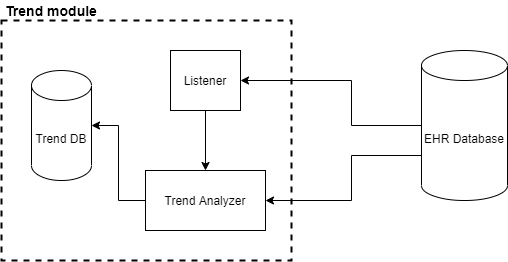
\includegraphics[scale = 0.45]{trend-module}
    \caption{An overview illustrating the Trend module}
    \label{fig:trend-module}
\end{figure}

As illustrated in Figure \ref{fig:trend-module}, this module would consist of three components. A listener listening for changes in the EHR database, a trend analyzer applying some algorithm to predict future values and a trend database to store this.

\begin{figure}[h]
    \centering
    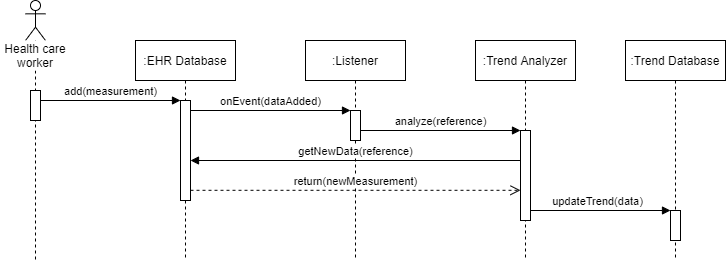
\includegraphics[scale = 0.45]{trend-sequence}
    \caption{A sequence diagram illustrating how the Trend module would work}
    \label{fig:trend-sequence}
\end{figure}

Figure \ref{fig:trend-sequence} illustrates how it would work. Since the computations required to make these predictions would be complex, it would be best to do them only once: when the data is added to the EHR Database. Then this data is stored in a separate database to be accessed by the Client Data Getter, seen in Figure \ref{fig:execution-view}, and could be used by the Rule Engine to prioritize patients. This data could also be used in combination with the patient specific data in the Patient View, to enable the care giver to get further insights into the health trends of the patient.

Due to the modularity of the code base, this module could be implemented without a major integration effort. It would require extending the functionality of the Rule Engine to take trends into account as well as extending the visualization components in the Patient View to display the trends.


\subsubsection{A more advanced notification log}
Twp simple notification logs are implemented in the system. The first contains information about all patients handled by the user and the second is a log for a specific patient. The second contains a full log of all events, but the overview notification log for all patients is simplified. Thus the simplified log could be improved and this is discussed below.

In the system now, after the overview data is retrieved to the overview module, this data is then passed to the notification log. The log displays date of the latest measurement added for a patient, as well as which measurements were added this date. It is only the last measurement for a patient that i displayed since it would be slow to send all data for every patient to the front end, and then have the front end derive notifications from this. A better solution would be an implementation closer to the Trend Analysis module, illustrated in Figure \ref{fig:notification-module}.

\begin{figure}[h]
    \centering
    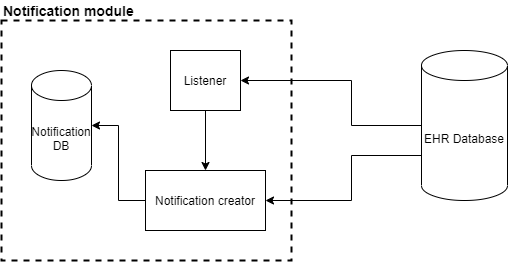
\includegraphics[scale = 0.45]{notification-module}
    \caption{An overview illustrating the improved Notification Module}
    \label{fig:notification-module}
\end{figure}

To improve the overview notification log, the functionality should be extended in the following way: A listener listens for changes in a patients EHR. When a change happens, a notification is created in a database. The notifications are also classified based on importance. A notification that e.g. a patient has changed his emergency contact would be prioritized below e.g. a patient has added a measurement that transitions the patient from one priority class to another in the Rule Engine. The entries in the database are then retrieved and loaded into the overview notification log. This enables the log to contain rich information, but does not significantly impair the performance and loading time. The notification could contain information such as:

\begin{description}
\item [Measurement added] A new measurement has been added.
\item [Measurement deviates] A measurement that was added deviates from the previous measurements. This could be flagged as suspected faulty, as something good or as something bad.
\item [Transition in priority class] If a passenger moves from low priority to high priority, this would be logged.
\item [Significant trend change] If integrated with the Trend Analyzer, a notification could be created when a new measurement changes the previous trend or prediction significantly.
\end{description}

Implementing this would require some effort in creating the listener, the component creating the notification and the integration with the Trend Analyzer if this module is also added. However, no major changes elsewhere are required. The front end already contains the functionality necessary to display any notification as well as prioritizing and sorting among notifications.

\subsubsection{Tweaking Rule Engine based on data set size}\label{future-prioritization}
As the number of patients increase, there is a high likelihood that the Rule Engine will prioritize a large number of patients as the highest priority. In this case it will be quite hard for a health care worker to prioritize between the patients. To handle this there are two possible approaches.

\begin{description}
\item [Dynamic prioritization] The absolute number of patients classified as the highest priority class is limited. Thus, only the e.g. 20 most critical patients are classified as the highest priority. This would help the system avoid notification fatigue in its users. 
\item [Non-integer prioritization] In the system now, the classifications are made in integers. One integer corresponds to one group of patients with a condition classified as equally serious. Non-integer prioritization would change this, and instead classify a patient's condition into a non-integer number greater than zero using some mathematical formula.
\end{description}

There are some problems with both approaches. The first creates a invalid view of the patients. If there are many critical patients, this would not be reflected in the overview as some would be classified as less severe. The second approach makes prioritization less clear as a number is harder to to judge a number than it is to judge a class, such as "Critical condition" or "Low priority".

The best solution would be a combination of the two. In this, the classification into priorities is dynamic so there is a fixed maximum number of patients in the most critical classes. However, next to the symbol representing the class the non-integer number is also displayed. Thus the user can both get a good overview with groups with a graphical symbol or color as well as a number so the user can differentiate between the members of each class. Implementing this would require a re-work of the Rule Engine as well as the database storing the custom rules for the Rule Engine. 

\section{Appendix}
\textbf{TODO:} Populate
\subsection{OpenEHR Templates}


\end{document}
